\documentclass[1p]{elsarticle_modified}
%\bibliographystyle{elsarticle-num}

%\usepackage[colorlinks]{hyperref}
%\usepackage{abbrmath_seonhwa} %\Abb, \Ascr, \Acal ,\Abf, \Afrak
\usepackage{amsfonts}
\usepackage{amssymb}
\usepackage{amsmath}
\usepackage{amsthm}
\usepackage{scalefnt}
\usepackage{amsbsy}
\usepackage{kotex}
\usepackage{caption}
\usepackage{subfig}
\usepackage{color}
\usepackage{graphicx}
\usepackage{xcolor} %% white, black, red, green, blue, cyan, magenta, yellow
\usepackage{float}
\usepackage{setspace}
\usepackage{hyperref}

\usepackage{tikz}
\usetikzlibrary{arrows}

\usepackage{multirow}
\usepackage{array} % fixed length table
\usepackage{hhline}

%%%%%%%%%%%%%%%%%%%%%
\makeatletter
\renewcommand*\env@matrix[1][\arraystretch]{%
	\edef\arraystretch{#1}%
	\hskip -\arraycolsep
	\let\@ifnextchar\new@ifnextchar
	\array{*\c@MaxMatrixCols c}}
\makeatother %https://tex.stackexchange.com/questions/14071/how-can-i-increase-the-line-spacing-in-a-matrix
%%%%%%%%%%%%%%%

\usepackage[normalem]{ulem}

\newcommand{\msout}[1]{\ifmmode\text{\sout{\ensuremath{#1}}}\else\sout{#1}\fi}
%SOURCE: \msout is \stkout macro in https://tex.stackexchange.com/questions/20609/strikeout-in-math-mode

\newcommand{\cancel}[1]{
	\ifmmode
	{\color{red}\msout{#1}}
	\else
	{\color{red}\sout{#1}}
	\fi
}

\newcommand{\add}[1]{
	{\color{blue}\uwave{#1}}
}

\newcommand{\replace}[2]{
	\ifmmode
	{\color{red}\msout{#1}}{\color{blue}\uwave{#2}}
	\else
	{\color{red}\sout{#1}}{\color{blue}\uwave{#2}}
	\fi
}

\newcommand{\Sol}{\mathcal{S}} %segment
\newcommand{\D}{D} %diagram
\newcommand{\A}{\mathcal{A}} %arc


%%%%%%%%%%%%%%%%%%%%%%%%%%%%%5 test

\def\sl{\operatorname{\textup{SL}}(2,\Cbb)}
\def\psl{\operatorname{\textup{PSL}}(2,\Cbb)}
\def\quan{\mkern 1mu \triangleright \mkern 1mu}

\theoremstyle{definition}
\newtheorem{thm}{Theorem}[section]
\newtheorem{prop}[thm]{Proposition}
\newtheorem{lem}[thm]{Lemma}
\newtheorem{ques}[thm]{Question}
\newtheorem{cor}[thm]{Corollary}
\newtheorem{defn}[thm]{Definition}
\newtheorem{exam}[thm]{Example}
\newtheorem{rmk}[thm]{Remark}
\newtheorem{alg}[thm]{Algorithm}

\newcommand{\I}{\sqrt{-1}}
\begin{document}

%\begin{frontmatter}
%
%\title{Boundary parabolic representations of knots up to 8 crossings}
%
%%% Group authors per affiliation:
%\author{Yunhi Cho} 
%\address{Department of Mathematics, University of Seoul, Seoul, Korea}
%\ead{yhcho@uos.ac.kr}
%
%
%\author{Seonhwa Kim} %\fnref{s_kim}}
%\address{Center for Geometry and Physics, Institute for Basic Science, Pohang, 37673, Korea}
%\ead{ryeona17@ibs.re.kr}
%
%\author{Hyuk Kim}
%\address{Department of Mathematical Sciences, Seoul National University, Seoul 08826, Korea}
%\ead{hyukkim@snu.ac.kr}
%
%\author{Seokbeom Yoon}
%\address{Department of Mathematical Sciences, Seoul National University, Seoul, 08826,  Korea}
%\ead{sbyoon15@snu.ac.kr}
%
%\begin{abstract}
%We find all boundary parabolic representation of knots up to 8 crossings.
%
%\end{abstract}
%\begin{keyword}
%    \MSC[2010] 57M25 
%\end{keyword}
%
%\end{frontmatter}

%\linenumbers
%\tableofcontents
%
\newcommand\colored[1]{\textcolor{white}{\rule[-0.35ex]{0.8em}{1.4ex}}\kern-0.8em\color{red} #1}%
%\newcommand\colored[1]{\textcolor{white}{ #1}\kern-2.17ex	\textcolor{white}{ #1}\kern-1.81ex	\textcolor{white}{ #1}\kern-2.15ex\color{red}#1	}

{\Large $\underline{11a_{244}~(K11a_{244})}$}

\setlength{\tabcolsep}{10pt}
\renewcommand{\arraystretch}{1.6}
\vspace{1cm}\begin{tabular}{m{100pt}>{\centering\arraybackslash}m{274pt}}
\multirow{5}{120pt}{
	\centering
	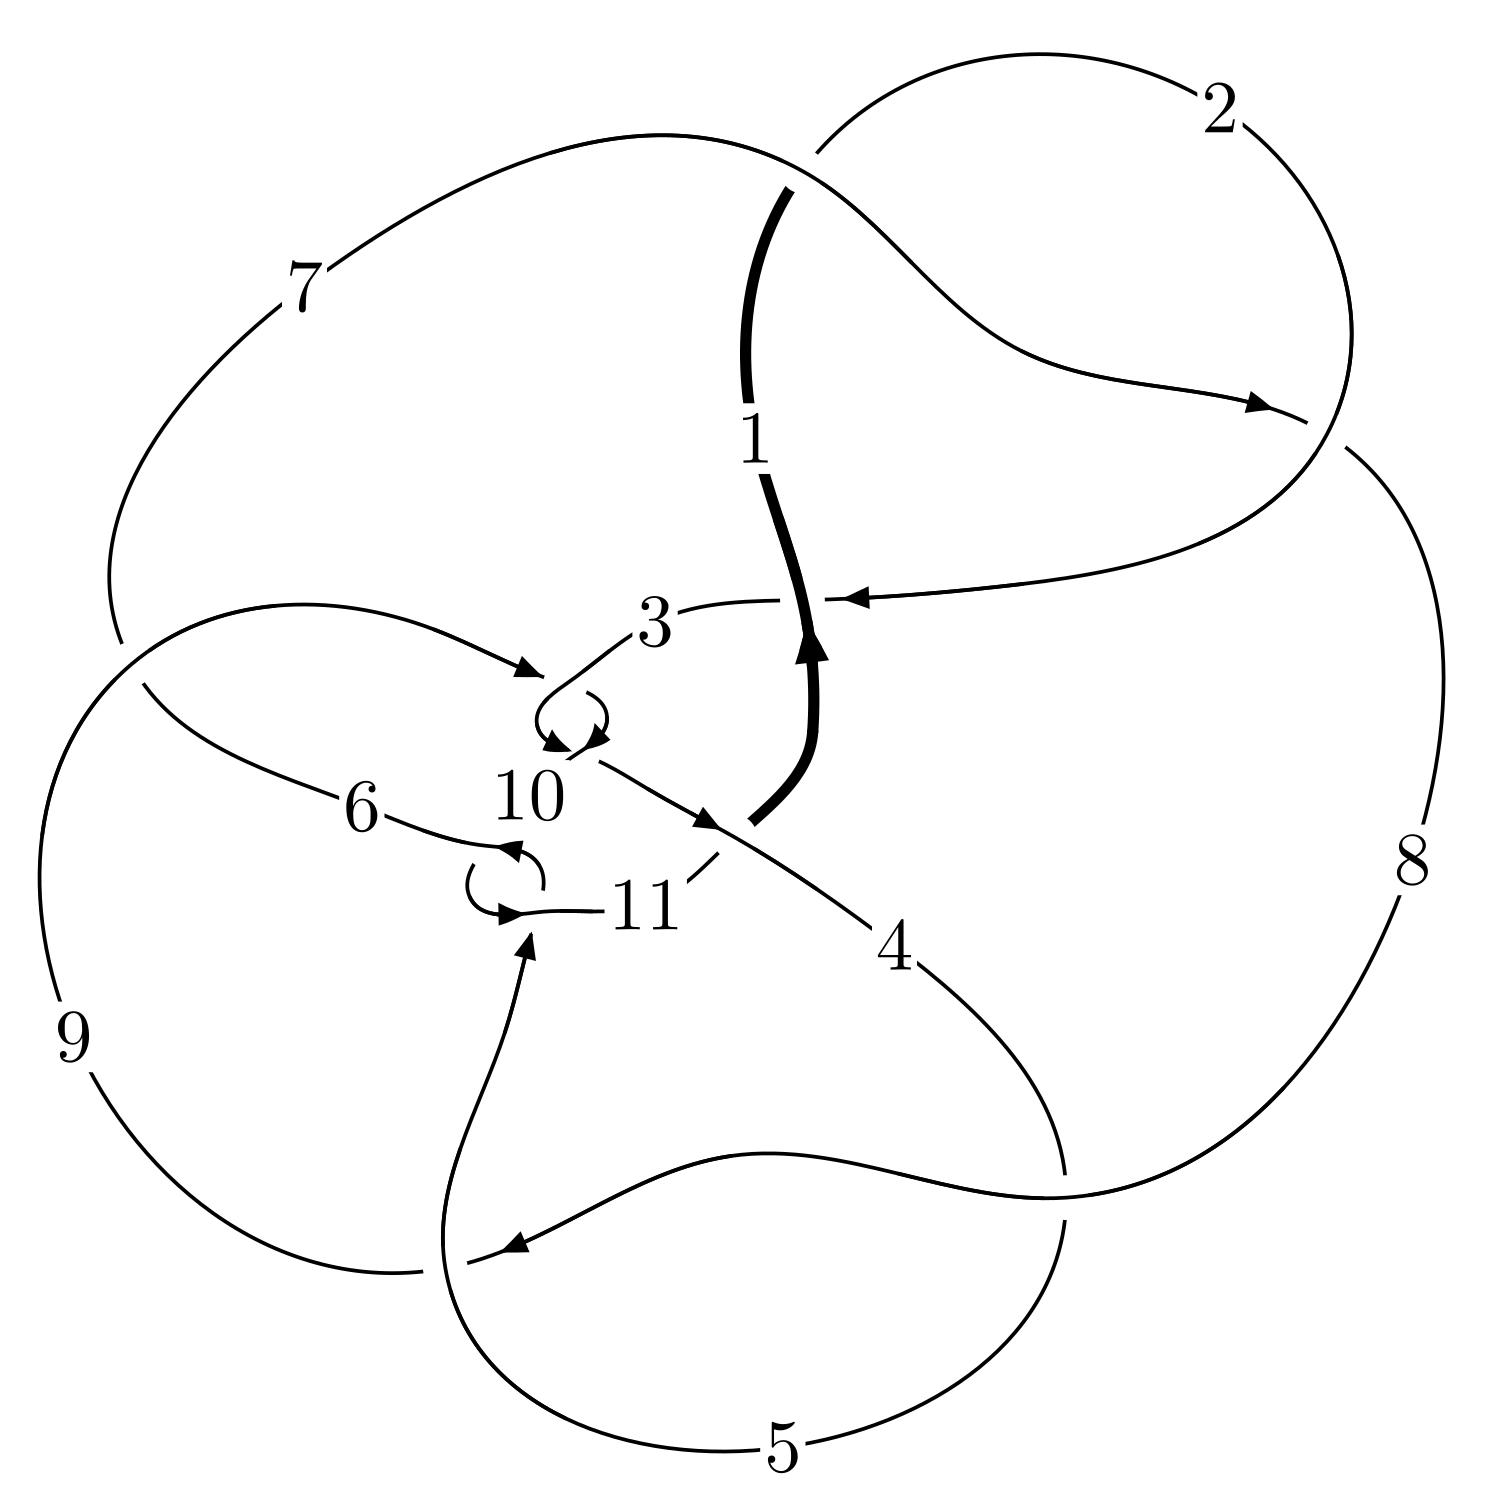
\includegraphics[width=112pt]{../../../GIT/diagram.site/Diagrams/png/493_11a_244.png}\\
\ \ \ A knot diagram\footnotemark}&
\allowdisplaybreaks
\textbf{Linearized knot diagam} \\
\cline{2-2}
 &
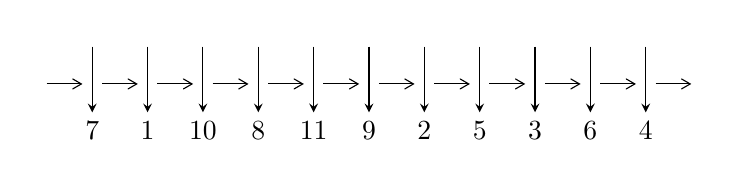
\begin{tikzpicture}[x=20pt, y=17pt]
	% nodes
	\node (C0) at (0, 0) {};
	\node (C1) at (1, 0) {};
	\node (C1U) at (1, +1) {};
	\node (C1D) at (1, -1) {7};

	\node (C2) at (2, 0) {};
	\node (C2U) at (2, +1) {};
	\node (C2D) at (2, -1) {1};

	\node (C3) at (3, 0) {};
	\node (C3U) at (3, +1) {};
	\node (C3D) at (3, -1) {10};

	\node (C4) at (4, 0) {};
	\node (C4U) at (4, +1) {};
	\node (C4D) at (4, -1) {8};

	\node (C5) at (5, 0) {};
	\node (C5U) at (5, +1) {};
	\node (C5D) at (5, -1) {11};

	\node (C6) at (6, 0) {};
	\node (C6U) at (6, +1) {};
	\node (C6D) at (6, -1) {9};

	\node (C7) at (7, 0) {};
	\node (C7U) at (7, +1) {};
	\node (C7D) at (7, -1) {2};

	\node (C8) at (8, 0) {};
	\node (C8U) at (8, +1) {};
	\node (C8D) at (8, -1) {5};

	\node (C9) at (9, 0) {};
	\node (C9U) at (9, +1) {};
	\node (C9D) at (9, -1) {3};

	\node (C10) at (10, 0) {};
	\node (C10U) at (10, +1) {};
	\node (C10D) at (10, -1) {6};

	\node (C11) at (11, 0) {};
	\node (C11U) at (11, +1) {};
	\node (C11D) at (11, -1) {4};
	\node (C12) at (12, 0) {};

	% arrows
	\draw[->,>={angle 60}]
	(C0) edge (C1) (C1) edge (C2) (C2) edge (C3) (C3) edge (C4) (C4) edge (C5) (C5) edge (C6) (C6) edge (C7) (C7) edge (C8) (C8) edge (C9) (C9) edge (C10) (C10) edge (C11) (C11) edge (C12) ;	\draw[->,>=stealth]
	(C1U) edge (C1D) (C2U) edge (C2D) (C3U) edge (C3D) (C4U) edge (C4D) (C5U) edge (C5D) (C6U) edge (C6D) (C7U) edge (C7D) (C8U) edge (C8D) (C9U) edge (C9D) (C10U) edge (C10D) (C11U) edge (C11D) ;
	\end{tikzpicture} \\
\hhline{~~} \\& 
\textbf{Solving Sequence} \\ \cline{2-2} 
 &
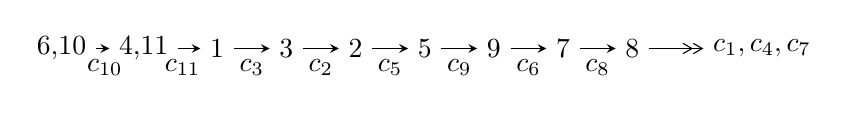
\begin{tikzpicture}[x=25pt, y=7pt]
	% node
	\node (A0) at (-1/8, 0) {6,10};
	\node (A1) at (17/16, 0) {4,11};
	\node (A2) at (17/8, 0) {1};
	\node (A3) at (25/8, 0) {3};
	\node (A4) at (33/8, 0) {2};
	\node (A5) at (41/8, 0) {5};
	\node (A6) at (49/8, 0) {9};
	\node (A7) at (57/8, 0) {7};
	\node (A8) at (65/8, 0) {8};
	\node (C1) at (1/2, -1) {$c_{10}$};
	\node (C2) at (13/8, -1) {$c_{11}$};
	\node (C3) at (21/8, -1) {$c_{3}$};
	\node (C4) at (29/8, -1) {$c_{2}$};
	\node (C5) at (37/8, -1) {$c_{5}$};
	\node (C6) at (45/8, -1) {$c_{9}$};
	\node (C7) at (53/8, -1) {$c_{6}$};
	\node (C8) at (61/8, -1) {$c_{8}$};
	\node (A9) at (10, 0) {$c_{1},c_{4},c_{7}$};

	% edge
	\draw[->,>=stealth]	
	(A0) edge (A1) (A1) edge (A2) (A2) edge (A3) (A3) edge (A4) (A4) edge (A5) (A5) edge (A6) (A6) edge (A7) (A7) edge (A8) ;
	\draw[->>,>={angle 60}]	
	(A8) edge (A9);
\end{tikzpicture} \\ 

\end{tabular} \\

\footnotetext{
The image of knot diagram is generated by the software ``\textbf{Draw programme}" developed by Andrew Bartholomew(\url{http://www.layer8.co.uk/maths/draw/index.htm\#Running-draw}), where we modified some parts for our purpose(\url{https://github.com/CATsTAILs/LinksPainter}).
}\phantom \\ \newline 
\centering \textbf{Ideals for irreducible components\footnotemark of $X_{\text{par}}$} 
 
\begin{align*}
I^u_{1}&=\langle 
-4.39064\times10^{39} u^{31}+4.83121\times10^{39} u^{30}+\cdots+3.73404\times10^{41} b+3.85648\times10^{41},\\
\phantom{I^u_{1}}&\phantom{= \langle  }5.47363\times10^{41} u^{31}-1.44531\times10^{42} u^{30}+\cdots+1.94170\times10^{43} a+9.06455\times10^{42},\\
\phantom{I^u_{1}}&\phantom{= \langle  }u^{32}-3 u^{31}+\cdots+114 u-26\rangle \\
I^u_{2}&=\langle 
2 u^{23} a+2 u^{23}+\cdots+3 a+2,\;4 u^{23} a-10 u^{23}+\cdots+4 a-8,\;u^{24}+u^{23}+\cdots+2 u+1\rangle \\
I^u_{3}&=\langle 
b+u,\;4 a^2-12 a u-2 a+3 u-8,\;u^2+1\rangle \\
I^u_{4}&=\langle 
b+1,\;6 a- u+2,\;u^2-2\rangle \\
\\
I^v_{1}&=\langle 
a,\;b-1,\;v+1\rangle \\
\end{align*}
\raggedright * 5 irreducible components of $\dim_{\mathbb{C}}=0$, with total 87 representations.\\
\footnotetext{All coefficients of polynomials are rational numbers. But the coefficients are sometimes approximated in decimal forms when there is not enough margin.}
\newpage
\renewcommand{\arraystretch}{1}
\centering \section*{I. $I^u_{1}= \langle -4.39\times10^{39} u^{31}+4.83\times10^{39} u^{30}+\cdots+3.73\times10^{41} b+3.86\times10^{41},\;5.47\times10^{41} u^{31}-1.45\times10^{42} u^{30}+\cdots+1.94\times10^{43} a+9.06\times10^{42},\;u^{32}-3 u^{31}+\cdots+114 u-26 \rangle$}
\flushleft \textbf{(i) Arc colorings}\\
\begin{tabular}{m{7pt} m{180pt} m{7pt} m{180pt} }
\flushright $a_{6}=$&$\begin{pmatrix}0\\u\end{pmatrix}$ \\
\flushright $a_{10}=$&$\begin{pmatrix}1\\0\end{pmatrix}$ \\
\flushright $a_{4}=$&$\begin{pmatrix}-0.0281899 u^{31}+0.0744353 u^{30}+\cdots+6.65054 u-0.466836\\0.0117584 u^{31}-0.0129383 u^{30}+\cdots+4.93202 u-1.03279\end{pmatrix}$ \\
\flushright $a_{11}=$&$\begin{pmatrix}1\\u^2\end{pmatrix}$ \\
\flushright $a_{1}=$&$\begin{pmatrix}0.0176665 u^{31}-0.0552376 u^{30}+\cdots+0.409548 u+0.504274\\0.00785720 u^{31}-0.0192778 u^{30}+\cdots+0.867861 u-0.446163\end{pmatrix}$ \\
\flushright $a_{3}=$&$\begin{pmatrix}-0.0164315 u^{31}+0.0614970 u^{30}+\cdots+11.5826 u-1.49963\\0.0117584 u^{31}-0.0129383 u^{30}+\cdots+4.93202 u-1.03279\end{pmatrix}$ \\
\flushright $a_{2}=$&$\begin{pmatrix}0.0234202 u^{31}-0.0628944 u^{30}+\cdots+8.74105 u-1.33147\\0.00391087 u^{31}+0.00194896 u^{30}+\cdots+1.97724 u-0.532828\end{pmatrix}$ \\
\flushright $a_{5}=$&$\begin{pmatrix}u\\u^3+u\end{pmatrix}$ \\
\flushright $a_{9}=$&$\begin{pmatrix}-0.0295883 u^{31}+0.0920957 u^{30}+\cdots+1.53443 u+1.13656\\0.0239060 u^{31}-0.0827478 u^{30}+\cdots-3.89581 u+0.819535\end{pmatrix}$ \\
\flushright $a_{7}=$&$\begin{pmatrix}0.0149220 u^{31}-0.0655790 u^{30}+\cdots-10.0660 u+1.54772\\-0.00696861 u^{31}+0.0183587 u^{30}+\cdots+1.25096 u-0.0818115\end{pmatrix}$ \\
\flushright $a_{8}=$&$\begin{pmatrix}-0.0519253 u^{31}+0.163878 u^{30}+\cdots+3.90769 u+0.830841\\0.0106080 u^{31}-0.0452849 u^{30}+\cdots-2.64731 u+0.637885\end{pmatrix}$\\ \flushright $a_{8}=$&$\begin{pmatrix}-0.0519253 u^{31}+0.163878 u^{30}+\cdots+3.90769 u+0.830841\\0.0106080 u^{31}-0.0452849 u^{30}+\cdots-2.64731 u+0.637885\end{pmatrix}$\\&\end{tabular}
\flushleft \textbf{(ii) Obstruction class $= -1$}\\~\\
\flushleft \textbf{(iii) Cusp Shapes $= -0.141620 u^{31}+0.504992 u^{30}+\cdots+51.3458 u-23.3173$}\\~\\
\newpage\renewcommand{\arraystretch}{1}
\flushleft \textbf{(iv) u-Polynomials at the component}\newline \\
\begin{tabular}{m{50pt}|m{274pt}}
Crossings & \hspace{64pt}u-Polynomials at each crossing \\
\hline $$\begin{aligned}c_{1},c_{7}\end{aligned}$$&$\begin{aligned}
&u^{32}+3 u^{31}+\cdots-46 u-10
\end{aligned}$\\
\hline $$\begin{aligned}c_{2}\end{aligned}$$&$\begin{aligned}
&u^{32}+17 u^{31}+\cdots+596 u+100
\end{aligned}$\\
\hline $$\begin{aligned}c_{3},c_{4},c_{8}\\c_{9}\end{aligned}$$&$\begin{aligned}
&u^{32}+u^{31}+\cdots-8 u-1
\end{aligned}$\\
\hline $$\begin{aligned}c_{5},c_{10}\end{aligned}$$&$\begin{aligned}
&u^{32}+3 u^{31}+\cdots-114 u-26
\end{aligned}$\\
\hline $$\begin{aligned}c_{6},c_{11}\end{aligned}$$&$\begin{aligned}
&16(16 u^{32}-32 u^{31}+\cdots+20 u+1)
\end{aligned}$\\
\hline
\end{tabular}\\~\\
\newpage\renewcommand{\arraystretch}{1}
\flushleft \textbf{(v) Riley Polynomials at the component}\newline \\
\begin{tabular}{m{50pt}|m{274pt}}
Crossings & \hspace{64pt}Riley Polynomials at each crossing \\
\hline $$\begin{aligned}c_{1},c_{7}\end{aligned}$$&$\begin{aligned}
&y^{32}-17 y^{31}+\cdots-596 y+100
\end{aligned}$\\
\hline $$\begin{aligned}c_{2}\end{aligned}$$&$\begin{aligned}
&y^{32}- y^{31}+\cdots-264816 y+10000
\end{aligned}$\\
\hline $$\begin{aligned}c_{3},c_{4},c_{8}\\c_{9}\end{aligned}$$&$\begin{aligned}
&y^{32}-11 y^{31}+\cdots-24 y+1
\end{aligned}$\\
\hline $$\begin{aligned}c_{5},c_{10}\end{aligned}$$&$\begin{aligned}
&y^{32}+13 y^{31}+\cdots+8740 y+676
\end{aligned}$\\
\hline $$\begin{aligned}c_{6},c_{11}\end{aligned}$$&$\begin{aligned}
&256(256 y^{32}+1664 y^{31}+\cdots-136 y+1)
\end{aligned}$\\
\hline
\end{tabular}\\~\\
\newpage\flushleft \textbf{(vi) Complex Volumes and Cusp Shapes}
$$\begin{array}{c|c|c}  
\text{Solutions to }I^u_{1}& \I (\text{vol} + \sqrt{-1}CS) & \text{Cusp shape}\\
 \hline 
\begin{aligned}
u &= -0.247680 + 0.984503 I \\
a &= \phantom{-}0.230631 + 0.815096 I \\
b &= \phantom{-}0.374640 + 0.105048 I\end{aligned}
 & \phantom{-}1.44688 - 2.10542 I & -10.64510 + 3.10426 I \\ \hline\begin{aligned}
u &= -0.247680 - 0.984503 I \\
a &= \phantom{-}0.230631 - 0.815096 I \\
b &= \phantom{-}0.374640 - 0.105048 I\end{aligned}
 & \phantom{-}1.44688 + 2.10542 I & -10.64510 - 3.10426 I \\ \hline\begin{aligned}
u &= \phantom{-}0.322065 + 1.002960 I \\
a &= -0.79959 + 1.57315 I \\
b &= \phantom{-}0.494847 - 1.304260 I\end{aligned}
 & \phantom{-}3.40906 - 3.86825 I & -10.66165 + 7.93865 I \\ \hline\begin{aligned}
u &= \phantom{-}0.322065 - 1.002960 I \\
a &= -0.79959 - 1.57315 I \\
b &= \phantom{-}0.494847 + 1.304260 I\end{aligned}
 & \phantom{-}3.40906 + 3.86825 I & -10.66165 - 7.93865 I \\ \hline\begin{aligned}
u &= \phantom{-}0.749051 + 0.842571 I \\
a &= \phantom{-}0.838998 - 0.649336 I \\
b &= \phantom{-}0.805918 + 0.420403 I\end{aligned}
 & \phantom{-}1.15662 - 1.21443 I & -10.34690 + 5.00886 I \\ \hline\begin{aligned}
u &= \phantom{-}0.749051 - 0.842571 I \\
a &= \phantom{-}0.838998 + 0.649336 I \\
b &= \phantom{-}0.805918 - 0.420403 I\end{aligned}
 & \phantom{-}1.15662 + 1.21443 I & -10.34690 - 5.00886 I \\ \hline\begin{aligned}
u &= -0.261685 + 1.100560 I \\
a &= \phantom{-}0.69752 + 1.32278 I \\
b &= -0.560070 - 1.085440 I\end{aligned}
 & \phantom{-}4.73730 - 0.53503 I & -5.59189 - 1.15953 I \\ \hline\begin{aligned}
u &= -0.261685 - 1.100560 I \\
a &= \phantom{-}0.69752 - 1.32278 I \\
b &= -0.560070 + 1.085440 I\end{aligned}
 & \phantom{-}4.73730 + 0.53503 I & -5.59189 + 1.15953 I \\ \hline\begin{aligned}
u &= \phantom{-}1.159410 + 0.253577 I \\
a &= -0.235640 - 0.264464 I \\
b &= -1.242110 + 0.484247 I\end{aligned}
 & -6.13645 + 10.98730 I & -16.3430 - 7.4849 I \\ \hline\begin{aligned}
u &= \phantom{-}1.159410 - 0.253577 I \\
a &= -0.235640 + 0.264464 I \\
b &= -1.242110 - 0.484247 I\end{aligned}
 & -6.13645 - 10.98730 I & -16.3430 + 7.4849 I\\
 \hline 
 \end{array}$$\newpage$$\begin{array}{c|c|c}  
\text{Solutions to }I^u_{1}& \I (\text{vol} + \sqrt{-1}CS) & \text{Cusp shape}\\
 \hline 
\begin{aligned}
u &= -1.140650 + 0.360946 I \\
a &= \phantom{-}0.307006 - 0.172337 I \\
b &= \phantom{-}1.128760 + 0.444978 I\end{aligned}
 & -3.38197 - 5.23032 I & -13.5291 + 4.8406 I \\ \hline\begin{aligned}
u &= -1.140650 - 0.360946 I \\
a &= \phantom{-}0.307006 + 0.172337 I \\
b &= \phantom{-}1.128760 - 0.444978 I\end{aligned}
 & -3.38197 + 5.23032 I & -13.5291 - 4.8406 I \\ \hline\begin{aligned}
u &= \phantom{-}0.141488 + 0.788388 I \\
a &= -0.36135 + 2.04053 I \\
b &= \phantom{-}0.099839 - 1.311650 I\end{aligned}
 & \phantom{-}2.29463 + 1.59601 I & -17.2362 + 0.3937 I \\ \hline\begin{aligned}
u &= \phantom{-}0.141488 - 0.788388 I \\
a &= -0.36135 - 2.04053 I \\
b &= \phantom{-}0.099839 + 1.311650 I\end{aligned}
 & \phantom{-}2.29463 - 1.59601 I & -17.2362 - 0.3937 I \\ \hline\begin{aligned}
u &= -0.736458 + 1.048230 I \\
a &= -0.625364 - 1.039090 I \\
b &= -0.962297 + 0.501826 I\end{aligned}
 & \phantom{-}1.70241 + 7.23076 I & -10.37930 - 9.14942 I \\ \hline\begin{aligned}
u &= -0.736458 - 1.048230 I \\
a &= -0.625364 + 1.039090 I \\
b &= -0.962297 - 0.501826 I\end{aligned}
 & \phantom{-}1.70241 - 7.23076 I & -10.37930 + 9.14942 I \\ \hline\begin{aligned}
u &= -0.097231 + 1.300930 I \\
a &= \phantom{-}0.428856 + 0.829956 I \\
b &= -0.638240 - 0.573688 I\end{aligned}
 & \phantom{-}3.55297 - 1.35902 I & -6.22009 + 3.91725 I \\ \hline\begin{aligned}
u &= -0.097231 - 1.300930 I \\
a &= \phantom{-}0.428856 - 0.829956 I \\
b &= -0.638240 + 0.573688 I\end{aligned}
 & \phantom{-}3.55297 + 1.35902 I & -6.22009 - 3.91725 I \\ \hline\begin{aligned}
u &= -0.66504 + 1.26287 I \\
a &= -0.08339 - 1.53240 I \\
b &= -1.242040 + 0.607992 I\end{aligned}
 & -0.46603 + 11.63550 I & -10.91066 - 6.70327 I \\ \hline\begin{aligned}
u &= -0.66504 - 1.26287 I \\
a &= -0.08339 + 1.53240 I \\
b &= -1.242040 - 0.607992 I\end{aligned}
 & -0.46603 - 11.63550 I & -10.91066 + 6.70327 I\\
 \hline 
 \end{array}$$\newpage$$\begin{array}{c|c|c}  
\text{Solutions to }I^u_{1}& \I (\text{vol} + \sqrt{-1}CS) & \text{Cusp shape}\\
 \hline 
\begin{aligned}
u &= \phantom{-}0.64627 + 1.29426 I \\
a &= -0.04894 - 1.63210 I \\
b &= \phantom{-}1.30934 + 0.63525 I\end{aligned}
 & -2.8457 - 17.3477 I & -13.2852 + 10.0205 I \\ \hline\begin{aligned}
u &= \phantom{-}0.64627 - 1.29426 I \\
a &= -0.04894 + 1.63210 I \\
b &= \phantom{-}1.30934 - 0.63525 I\end{aligned}
 & -2.8457 + 17.3477 I & -13.2852 - 10.0205 I \\ \hline\begin{aligned}
u &= \phantom{-}1.38769 + 0.52320 I \\
a &= -0.203571 - 0.024919 I \\
b &= -1.092060 + 0.243675 I\end{aligned}
 & -9.14170 + 1.02273 I & -18.9526 - 6.3910 I \\ \hline\begin{aligned}
u &= \phantom{-}1.38769 - 0.52320 I \\
a &= -0.203571 + 0.024919 I \\
b &= -1.092060 - 0.243675 I\end{aligned}
 & -9.14170 - 1.02273 I & -18.9526 + 6.3910 I \\ \hline\begin{aligned}
u &= \phantom{-}0.75214 + 1.28922 I \\
a &= -0.023703 - 1.211370 I \\
b &= \phantom{-}1.242430 + 0.458182 I\end{aligned}
 & -6.39323 - 8.37491 I & -16.6922 + 6.0879 I \\ \hline\begin{aligned}
u &= \phantom{-}0.75214 - 1.28922 I \\
a &= -0.023703 + 1.211370 I \\
b &= \phantom{-}1.242430 - 0.458182 I\end{aligned}
 & -6.39323 + 8.37491 I & -16.6922 - 6.0879 I \\ \hline\begin{aligned}
u &= \phantom{-}0.15834 + 1.54684 I \\
a &= -0.519510 + 0.469576 I \\
b &= \phantom{-}0.921773 - 0.411908 I\end{aligned}
 & \phantom{-}0.43477 + 5.74906 I & -12.0210 - 8.3466 I \\ \hline\begin{aligned}
u &= \phantom{-}0.15834 - 1.54684 I \\
a &= -0.519510 - 0.469576 I \\
b &= \phantom{-}0.921773 + 0.411908 I\end{aligned}
 & \phantom{-}0.43477 - 5.74906 I & -12.0210 + 8.3466 I \\ \hline\begin{aligned}
u &= -1.61248\phantom{ +0.000000I} \\
a &= -0.366965\phantom{ +0.000000I} \\
b &= -0.861180\phantom{ +0.000000I}\end{aligned}
 & -7.60439\phantom{ +0.000000I} & -2.56870\phantom{ +0.000000I} \\ \hline\begin{aligned}
u &= -0.027688 + 0.377024 I \\
a &= \phantom{-}0.62467 + 1.38038 I \\
b &= \phantom{-}0.136888 + 0.524281 I\end{aligned}
 & \phantom{-}1.38354 - 2.30080 I & -9.19830 + 4.85013 I\\
 \hline 
 \end{array}$$\newpage$$\begin{array}{c|c|c}  
\text{Solutions to }I^u_{1}& \I (\text{vol} + \sqrt{-1}CS) & \text{Cusp shape}\\
 \hline 
\begin{aligned}
u &= -0.027688 - 0.377024 I \\
a &= \phantom{-}0.62467 - 1.38038 I \\
b &= \phantom{-}0.136888 - 0.524281 I\end{aligned}
 & \phantom{-}1.38354 + 2.30080 I & -9.19830 - 4.85013 I \\ \hline\begin{aligned}
u &= \phantom{-}0.332429\phantom{ +0.000000I} \\
a &= \phantom{-}0.529099\phantom{ +0.000000I} \\
b &= \phantom{-}0.305964\phantom{ +0.000000I}\end{aligned}
 & -0.575721\phantom{ +0.000000I} & -17.4050\phantom{ +0.000000I}\\
 \hline 
 \end{array}$$\newpage\newpage\renewcommand{\arraystretch}{1}
\centering \section*{II. $I^u_{2}= \langle 2 u^{23} a+2 u^{23}+\cdots+3 a+2,\;4 u^{23} a-10 u^{23}+\cdots+4 a-8,\;u^{24}+u^{23}+\cdots+2 u+1 \rangle$}
\flushleft \textbf{(i) Arc colorings}\\
\begin{tabular}{m{7pt} m{180pt} m{7pt} m{180pt} }
\flushright $a_{6}=$&$\begin{pmatrix}0\\u\end{pmatrix}$ \\
\flushright $a_{10}=$&$\begin{pmatrix}1\\0\end{pmatrix}$ \\
\flushright $a_{4}=$&$\begin{pmatrix}a\\-2 u^{23} a-2 u^{23}+\cdots-3 a-2\end{pmatrix}$ \\
\flushright $a_{11}=$&$\begin{pmatrix}1\\u^2\end{pmatrix}$ \\
\flushright $a_{1}=$&$\begin{pmatrix}-2 u^{22} a+12 u^{23}+\cdots+2 a+11\\2 u^{22}+2 u^{21}+\cdots+4 u+5\end{pmatrix}$ \\
\flushright $a_{3}=$&$\begin{pmatrix}-2 u^{23} a-2 u^{23}+\cdots-2 a-2\\-2 u^{23} a-2 u^{23}+\cdots-3 a-2\end{pmatrix}$ \\
\flushright $a_{2}=$&$\begin{pmatrix}-2 u^{22} a-2 u^{23}+\cdots- a+12\\-2 u^{23} a-4 u^{23}+\cdots-3 a-2\end{pmatrix}$ \\
\flushright $a_{5}=$&$\begin{pmatrix}u\\u^3+u\end{pmatrix}$ \\
\flushright $a_{9}=$&$\begin{pmatrix}-3 u^{23} a-2 u^{23}+\cdots-4 a-6\\- u^{23} a-2 u^{23}+\cdots-2 a-4\end{pmatrix}$ \\
\flushright $a_{7}=$&$\begin{pmatrix}2 u^{23} a-8 u^{23}+\cdots-2 a+10\\2 u^{23} a+u^{22} a+\cdots+3 a+2\end{pmatrix}$ \\
\flushright $a_{8}=$&$\begin{pmatrix}-2 u^{23} a- u^{22}+\cdots-2 a-4\\-1\end{pmatrix}$\\ \flushright $a_{8}=$&$\begin{pmatrix}-2 u^{23} a- u^{22}+\cdots-2 a-4\\-1\end{pmatrix}$\\&\end{tabular}
\flushleft \textbf{(ii) Obstruction class $= -1$}\\~\\
\flushleft \textbf{(iii) Cusp Shapes $= -4 u^{23}-4 u^{22}-24 u^{21}-20 u^{20}-68 u^{19}-52 u^{18}-108 u^{17}-80 u^{16}-96 u^{15}-84 u^{14}-32 u^{13}-52 u^{12}+24 u^{11}-8 u^{10}+32 u^9+28 u^8+16 u^7+20 u^6+4 u^4+4 u^3-4 u^2-4 u-18$}\\~\\
\newpage\renewcommand{\arraystretch}{1}
\flushleft \textbf{(iv) u-Polynomials at the component}\newline \\
\begin{tabular}{m{50pt}|m{274pt}}
Crossings & \hspace{64pt}u-Polynomials at each crossing \\
\hline $$\begin{aligned}c_{1},c_{7}\end{aligned}$$&$\begin{aligned}
&(u^{24}- u^{23}+\cdots-2 u^3+1)^{2}
\end{aligned}$\\
\hline $$\begin{aligned}c_{2}\end{aligned}$$&$\begin{aligned}
&(u^{24}+11 u^{23}+\cdots-2 u^2+1)^{2}
\end{aligned}$\\
\hline $$\begin{aligned}c_{3},c_{4},c_{8}\\c_{9}\end{aligned}$$&$\begin{aligned}
&u^{48}+u^{47}+\cdots+60 u+17
\end{aligned}$\\
\hline $$\begin{aligned}c_{5},c_{10}\end{aligned}$$&$\begin{aligned}
&(u^{24}- u^{23}+\cdots-2 u+1)^{2}
\end{aligned}$\\
\hline $$\begin{aligned}c_{6},c_{11}\end{aligned}$$&$\begin{aligned}
&u^{48}+19 u^{47}+\cdots-5852 u+617
\end{aligned}$\\
\hline
\end{tabular}\\~\\
\newpage\renewcommand{\arraystretch}{1}
\flushleft \textbf{(v) Riley Polynomials at the component}\newline \\
\begin{tabular}{m{50pt}|m{274pt}}
Crossings & \hspace{64pt}Riley Polynomials at each crossing \\
\hline $$\begin{aligned}c_{1},c_{7}\end{aligned}$$&$\begin{aligned}
&(y^{24}-11 y^{23}+\cdots-2 y^2+1)^{2}
\end{aligned}$\\
\hline $$\begin{aligned}c_{2}\end{aligned}$$&$\begin{aligned}
&(y^{24}+5 y^{23}+\cdots-4 y+1)^{2}
\end{aligned}$\\
\hline $$\begin{aligned}c_{3},c_{4},c_{8}\\c_{9}\end{aligned}$$&$\begin{aligned}
&y^{48}-29 y^{47}+\cdots-2036 y+289
\end{aligned}$\\
\hline $$\begin{aligned}c_{5},c_{10}\end{aligned}$$&$\begin{aligned}
&(y^{24}+13 y^{23}+\cdots-2 y^2+1)^{2}
\end{aligned}$\\
\hline $$\begin{aligned}c_{6},c_{11}\end{aligned}$$&$\begin{aligned}
&y^{48}-17 y^{47}+\cdots+4462208 y+380689
\end{aligned}$\\
\hline
\end{tabular}\\~\\
\newpage\flushleft \textbf{(vi) Complex Volumes and Cusp Shapes}
$$\begin{array}{c|c|c}  
\text{Solutions to }I^u_{2}& \I (\text{vol} + \sqrt{-1}CS) & \text{Cusp shape}\\
 \hline 
\begin{aligned}
u &= \phantom{-}0.539628 + 0.849352 I \\
a &= \phantom{-}0.543922 + 0.247508 I \\
b &= -1.51045 + 0.21810 I\end{aligned}
 & -5.72979 - 5.71321 I & -16.1082 + 7.5036 I \\ \hline\begin{aligned}
u &= \phantom{-}0.539628 + 0.849352 I \\
a &= -0.33191 - 2.03598 I \\
b &= \phantom{-}1.039360 + 0.760521 I\end{aligned}
 & -5.72979 - 5.71321 I & -16.1082 + 7.5036 I \\ \hline\begin{aligned}
u &= \phantom{-}0.539628 - 0.849352 I \\
a &= \phantom{-}0.543922 - 0.247508 I \\
b &= -1.51045 - 0.21810 I\end{aligned}
 & -5.72979 + 5.71321 I & -16.1082 - 7.5036 I \\ \hline\begin{aligned}
u &= \phantom{-}0.539628 - 0.849352 I \\
a &= -0.33191 + 2.03598 I \\
b &= \phantom{-}1.039360 - 0.760521 I\end{aligned}
 & -5.72979 + 5.71321 I & -16.1082 - 7.5036 I \\ \hline\begin{aligned}
u &= -0.096397 + 0.986281 I \\
a &= \phantom{-}4.87120 + 4.00215 I \\
b &= \phantom{-}1.080380 + 0.019593 I\end{aligned}
 & -1.54603 + 2.05721 I & -7.72702 - 4.01793 I \\ \hline\begin{aligned}
u &= -0.096397 + 0.986281 I \\
a &= \phantom{-}4.84423 - 6.02369 I \\
b &= -0.896362 + 0.034778 I\end{aligned}
 & -1.54603 + 2.05721 I & -7.72702 - 4.01793 I \\ \hline\begin{aligned}
u &= -0.096397 - 0.986281 I \\
a &= \phantom{-}4.87120 - 4.00215 I \\
b &= \phantom{-}1.080380 - 0.019593 I\end{aligned}
 & -1.54603 - 2.05721 I & -7.72702 + 4.01793 I \\ \hline\begin{aligned}
u &= -0.096397 - 0.986281 I \\
a &= \phantom{-}4.84423 + 6.02369 I \\
b &= -0.896362 - 0.034778 I\end{aligned}
 & -1.54603 - 2.05721 I & -7.72702 + 4.01793 I \\ \hline\begin{aligned}
u &= -0.414627 + 0.808476 I \\
a &= \phantom{-}0.00257518 - 0.01121480 I \\
b &= \phantom{-}1.306580 + 0.198887 I\end{aligned}
 & -3.23391 + 1.77225 I & -11.98912 - 4.04184 I \\ \hline\begin{aligned}
u &= -0.414627 + 0.808476 I \\
a &= \phantom{-}0.35931 - 2.22876 I \\
b &= -0.979446 + 0.498112 I\end{aligned}
 & -3.23391 + 1.77225 I & -11.98912 - 4.04184 I\\
 \hline 
 \end{array}$$\newpage$$\begin{array}{c|c|c}  
\text{Solutions to }I^u_{2}& \I (\text{vol} + \sqrt{-1}CS) & \text{Cusp shape}\\
 \hline 
\begin{aligned}
u &= -0.414627 - 0.808476 I \\
a &= \phantom{-}0.00257518 + 0.01121480 I \\
b &= \phantom{-}1.306580 - 0.198887 I\end{aligned}
 & -3.23391 - 1.77225 I & -11.98912 + 4.04184 I \\ \hline\begin{aligned}
u &= -0.414627 - 0.808476 I \\
a &= \phantom{-}0.35931 + 2.22876 I \\
b &= -0.979446 - 0.498112 I\end{aligned}
 & -3.23391 - 1.77225 I & -11.98912 + 4.04184 I \\ \hline\begin{aligned}
u &= \phantom{-}0.542169 + 0.664263 I \\
a &= \phantom{-}0.666243 - 0.437409 I \\
b &= -1.306800 + 0.469542 I\end{aligned}
 & -6.25412 + 1.34320 I & -18.0296 - 0.6200 I \\ \hline\begin{aligned}
u &= \phantom{-}0.542169 + 0.664263 I \\
a &= -0.14319 - 1.94467 I \\
b &= \phantom{-}1.290650 + 0.487392 I\end{aligned}
 & -6.25412 + 1.34320 I & -18.0296 - 0.6200 I \\ \hline\begin{aligned}
u &= \phantom{-}0.542169 - 0.664263 I \\
a &= \phantom{-}0.666243 + 0.437409 I \\
b &= -1.306800 - 0.469542 I\end{aligned}
 & -6.25412 - 1.34320 I & -18.0296 + 0.6200 I \\ \hline\begin{aligned}
u &= \phantom{-}0.542169 - 0.664263 I \\
a &= -0.14319 + 1.94467 I \\
b &= \phantom{-}1.290650 - 0.487392 I\end{aligned}
 & -6.25412 - 1.34320 I & -18.0296 + 0.6200 I \\ \hline\begin{aligned}
u &= -0.796432 + 0.144602 I \\
a &= -0.786039 - 0.575477 I \\
b &= -0.017969 + 0.851963 I\end{aligned}
 & -2.49287 - 6.17959 I & -13.7852 + 5.0455 I \\ \hline\begin{aligned}
u &= -0.796432 + 0.144602 I \\
a &= -0.197166 - 0.175593 I \\
b &= -1.233680 - 0.435221 I\end{aligned}
 & -2.49287 - 6.17959 I & -13.7852 + 5.0455 I \\ \hline\begin{aligned}
u &= -0.796432 - 0.144602 I \\
a &= -0.786039 + 0.575477 I \\
b &= -0.017969 - 0.851963 I\end{aligned}
 & -2.49287 + 6.17959 I & -13.7852 - 5.0455 I \\ \hline\begin{aligned}
u &= -0.796432 - 0.144602 I \\
a &= -0.197166 + 0.175593 I \\
b &= -1.233680 + 0.435221 I\end{aligned}
 & -2.49287 + 6.17959 I & -13.7852 - 5.0455 I\\
 \hline 
 \end{array}$$\newpage$$\begin{array}{c|c|c}  
\text{Solutions to }I^u_{2}& \I (\text{vol} + \sqrt{-1}CS) & \text{Cusp shape}\\
 \hline 
\begin{aligned}
u &= -0.472424 + 1.121720 I \\
a &= -0.004693 - 1.220150 I \\
b &= -0.070699 + 0.850066 I\end{aligned}
 & -2.54173 + 3.77265 I & -13.8919 - 3.4911 I \\ \hline\begin{aligned}
u &= -0.472424 + 1.121720 I \\
a &= -0.225989 + 1.326630 I \\
b &= \phantom{-}1.276130 - 0.388706 I\end{aligned}
 & -2.54173 + 3.77265 I & -13.8919 - 3.4911 I \\ \hline\begin{aligned}
u &= -0.472424 - 1.121720 I \\
a &= -0.004693 + 1.220150 I \\
b &= -0.070699 - 0.850066 I\end{aligned}
 & -2.54173 - 3.77265 I & -13.8919 + 3.4911 I \\ \hline\begin{aligned}
u &= -0.472424 - 1.121720 I \\
a &= -0.225989 - 1.326630 I \\
b &= \phantom{-}1.276130 + 0.388706 I\end{aligned}
 & -2.54173 - 3.77265 I & -13.8919 + 3.4911 I \\ \hline\begin{aligned}
u &= \phantom{-}0.766849 + 0.083191 I \\
a &= \phantom{-}0.769852 - 0.382628 I \\
b &= \phantom{-}0.169700 + 0.594156 I\end{aligned}
 & -0.655501 + 1.182900 I & -10.60754 - 0.39910 I \\ \hline\begin{aligned}
u &= \phantom{-}0.766849 + 0.083191 I \\
a &= \phantom{-}0.400701 - 0.069987 I \\
b &= \phantom{-}1.032180 - 0.364777 I\end{aligned}
 & -0.655501 + 1.182900 I & -10.60754 - 0.39910 I \\ \hline\begin{aligned}
u &= \phantom{-}0.766849 - 0.083191 I \\
a &= \phantom{-}0.769852 + 0.382628 I \\
b &= \phantom{-}0.169700 - 0.594156 I\end{aligned}
 & -0.655501 - 1.182900 I & -10.60754 + 0.39910 I \\ \hline\begin{aligned}
u &= \phantom{-}0.766849 - 0.083191 I \\
a &= \phantom{-}0.400701 + 0.069987 I \\
b &= \phantom{-}1.032180 + 0.364777 I\end{aligned}
 & -0.655501 - 1.182900 I & -10.60754 + 0.39910 I \\ \hline\begin{aligned}
u &= -0.376287 + 1.204930 I \\
a &= \phantom{-}0.475135 + 0.983255 I \\
b &= \phantom{-}0.513121 - 0.339665 I\end{aligned}
 & \phantom{-}1.53995 - 2.24524 I & -8.97303 + 1.89383 I \\ \hline\begin{aligned}
u &= -0.376287 + 1.204930 I \\
a &= -0.408284 + 0.298929 I \\
b &= \phantom{-}0.696267 + 0.307021 I\end{aligned}
 & \phantom{-}1.53995 - 2.24524 I & -8.97303 + 1.89383 I\\
 \hline 
 \end{array}$$\newpage$$\begin{array}{c|c|c}  
\text{Solutions to }I^u_{2}& \I (\text{vol} + \sqrt{-1}CS) & \text{Cusp shape}\\
 \hline 
\begin{aligned}
u &= -0.376287 - 1.204930 I \\
a &= \phantom{-}0.475135 - 0.983255 I \\
b &= \phantom{-}0.513121 + 0.339665 I\end{aligned}
 & \phantom{-}1.53995 + 2.24524 I & -8.97303 - 1.89383 I \\ \hline\begin{aligned}
u &= -0.376287 - 1.204930 I \\
a &= -0.408284 - 0.298929 I \\
b &= \phantom{-}0.696267 - 0.307021 I\end{aligned}
 & \phantom{-}1.53995 + 2.24524 I & -8.97303 - 1.89383 I \\ \hline\begin{aligned}
u &= \phantom{-}0.413902 + 1.197930 I \\
a &= -0.198548 + 1.325430 I \\
b &= -0.820849 - 0.486407 I\end{aligned}
 & \phantom{-}3.07007 - 2.92383 I & -6.70980 + 3.29300 I \\ \hline\begin{aligned}
u &= \phantom{-}0.413902 + 1.197930 I \\
a &= \phantom{-}0.375753 - 0.333805 I \\
b &= -0.476232 + 0.580933 I\end{aligned}
 & \phantom{-}3.07007 - 2.92383 I & -6.70980 + 3.29300 I \\ \hline\begin{aligned}
u &= \phantom{-}0.413902 - 1.197930 I \\
a &= -0.198548 - 1.325430 I \\
b &= -0.820849 + 0.486407 I\end{aligned}
 & \phantom{-}3.07007 + 2.92383 I & -6.70980 - 3.29300 I \\ \hline\begin{aligned}
u &= \phantom{-}0.413902 - 1.197930 I \\
a &= \phantom{-}0.375753 + 0.333805 I \\
b &= -0.476232 - 0.580933 I\end{aligned}
 & \phantom{-}3.07007 + 2.92383 I & -6.70980 - 3.29300 I \\ \hline\begin{aligned}
u &= \phantom{-}0.486243 + 1.189530 I \\
a &= \phantom{-}0.531403 - 1.075720 I \\
b &= -0.278243 + 1.022640 I\end{aligned}
 & \phantom{-}2.55519 - 5.78082 I & -7.62473 + 3.72629 I \\ \hline\begin{aligned}
u &= \phantom{-}0.486243 + 1.189530 I \\
a &= \phantom{-}0.12458 + 1.60566 I \\
b &= -1.184610 - 0.672538 I\end{aligned}
 & \phantom{-}2.55519 - 5.78082 I & -7.62473 + 3.72629 I \\ \hline\begin{aligned}
u &= \phantom{-}0.486243 - 1.189530 I \\
a &= \phantom{-}0.531403 + 1.075720 I \\
b &= -0.278243 - 1.022640 I\end{aligned}
 & \phantom{-}2.55519 + 5.78082 I & -7.62473 - 3.72629 I \\ \hline\begin{aligned}
u &= \phantom{-}0.486243 - 1.189530 I \\
a &= \phantom{-}0.12458 - 1.60566 I \\
b &= -1.184610 + 0.672538 I\end{aligned}
 & \phantom{-}2.55519 + 5.78082 I & -7.62473 - 3.72629 I\\
 \hline 
 \end{array}$$\newpage$$\begin{array}{c|c|c}  
\text{Solutions to }I^u_{2}& \I (\text{vol} + \sqrt{-1}CS) & \text{Cusp shape}\\
 \hline 
\begin{aligned}
u &= -0.512242 + 1.189930 I \\
a &= -0.590726 - 1.274840 I \\
b &= \phantom{-}0.228910 + 1.166680 I\end{aligned}
 & \phantom{-}0.58237 + 11.00000 I & -10.68175 - 8.05284 I \\ \hline\begin{aligned}
u &= -0.512242 + 1.189930 I \\
a &= -0.24364 + 1.67429 I \\
b &= \phantom{-}1.30033 - 0.72492 I\end{aligned}
 & \phantom{-}0.58237 + 11.00000 I & -10.68175 - 8.05284 I \\ \hline\begin{aligned}
u &= -0.512242 - 1.189930 I \\
a &= -0.590726 + 1.274840 I \\
b &= \phantom{-}0.228910 - 1.166680 I\end{aligned}
 & \phantom{-}0.58237 - 11.00000 I & -10.68175 + 8.05284 I \\ \hline\begin{aligned}
u &= -0.512242 - 1.189930 I \\
a &= -0.24364 - 1.67429 I \\
b &= \phantom{-}1.30033 + 0.72492 I\end{aligned}
 & \phantom{-}0.58237 - 11.00000 I & -10.68175 + 8.05284 I \\ \hline\begin{aligned}
u &= -0.580381 + 0.259924 I \\
a &= -0.625985 - 0.961812 I \\
b &= -1.295020 - 0.005614 I\end{aligned}
 & -5.03285 + 0.40841 I & -17.8720 - 0.7556 I \\ \hline\begin{aligned}
u &= -0.580381 + 0.259924 I \\
a &= -1.20872 - 0.75067 I \\
b &= \phantom{-}0.636772 + 0.510637 I\end{aligned}
 & -5.03285 + 0.40841 I & -17.8720 - 0.7556 I \\ \hline\begin{aligned}
u &= -0.580381 - 0.259924 I \\
a &= -0.625985 + 0.961812 I \\
b &= -1.295020 + 0.005614 I\end{aligned}
 & -5.03285 - 0.40841 I & -17.8720 + 0.7556 I \\ \hline\begin{aligned}
u &= -0.580381 - 0.259924 I \\
a &= -1.20872 + 0.75067 I \\
b &= \phantom{-}0.636772 - 0.510637 I\end{aligned}
 & -5.03285 - 0.40841 I & -17.8720 + 0.7556 I\\
 \hline 
 \end{array}$$\newpage\newpage\renewcommand{\arraystretch}{1}
\centering \section*{III. $I^u_{3}= \langle b+u,\;4 a^2-12 a u-2 a+3 u-8,\;u^2+1 \rangle$}
\flushleft \textbf{(i) Arc colorings}\\
\begin{tabular}{m{7pt} m{180pt} m{7pt} m{180pt} }
\flushright $a_{6}=$&$\begin{pmatrix}0\\u\end{pmatrix}$ \\
\flushright $a_{10}=$&$\begin{pmatrix}1\\0\end{pmatrix}$ \\
\flushright $a_{4}=$&$\begin{pmatrix}a\\- u\end{pmatrix}$ \\
\flushright $a_{11}=$&$\begin{pmatrix}1\\-1\end{pmatrix}$ \\
\flushright $a_{1}=$&$\begin{pmatrix}2 a u+\frac{1}{2} a-\frac{3}{4} u+3\\- a u-2\end{pmatrix}$ \\
\flushright $a_{3}=$&$\begin{pmatrix}a- u\\- u\end{pmatrix}$ \\
\flushright $a_{2}=$&$\begin{pmatrix}2 a u+\frac{3}{2} a-\frac{11}{4} u+\frac{11}{4}\\- a u- a+u-\frac{3}{2}\end{pmatrix}$ \\
\flushright $a_{5}=$&$\begin{pmatrix}u\\0\end{pmatrix}$ \\
\flushright $a_{9}=$&$\begin{pmatrix}a u+2\\1\end{pmatrix}$ \\
\flushright $a_{7}=$&$\begin{pmatrix}\frac{1}{2} a u+a-2 u+\frac{3}{4}\\a- u\end{pmatrix}$ \\
\flushright $a_{8}=$&$\begin{pmatrix}a u+1\\1\end{pmatrix}$\\ \flushright $a_{8}=$&$\begin{pmatrix}a u+1\\1\end{pmatrix}$\\&\end{tabular}
\flushleft \textbf{(ii) Obstruction class $= 1$}\\~\\
\flushleft \textbf{(iii) Cusp Shapes $= 8 a-12 u-8$}\\~\\
\newpage\renewcommand{\arraystretch}{1}
\flushleft \textbf{(iv) u-Polynomials at the component}\newline \\
\begin{tabular}{m{50pt}|m{274pt}}
Crossings & \hspace{64pt}u-Polynomials at each crossing \\
\hline $$\begin{aligned}c_{1},c_{7}\end{aligned}$$&$\begin{aligned}
&u^4- u^2+1
\end{aligned}$\\
\hline $$\begin{aligned}c_{2}\end{aligned}$$&$\begin{aligned}
&(u^2+u+1)^2
\end{aligned}$\\
\hline $$\begin{aligned}c_{3},c_{4},c_{5}\\c_{8},c_{9},c_{10}\end{aligned}$$&$\begin{aligned}
&(u^2+1)^2
\end{aligned}$\\
\hline $$\begin{aligned}c_{6},c_{11}\end{aligned}$$&$\begin{aligned}
&16(16 u^4-16 u^3+20 u^2-8 u+1)
\end{aligned}$\\
\hline
\end{tabular}\\~\\
\newpage\renewcommand{\arraystretch}{1}
\flushleft \textbf{(v) Riley Polynomials at the component}\newline \\
\begin{tabular}{m{50pt}|m{274pt}}
Crossings & \hspace{64pt}Riley Polynomials at each crossing \\
\hline $$\begin{aligned}c_{1},c_{7}\end{aligned}$$&$\begin{aligned}
&(y^2- y+1)^2
\end{aligned}$\\
\hline $$\begin{aligned}c_{2}\end{aligned}$$&$\begin{aligned}
&(y^2+y+1)^2
\end{aligned}$\\
\hline $$\begin{aligned}c_{3},c_{4},c_{5}\\c_{8},c_{9},c_{10}\end{aligned}$$&$\begin{aligned}
&(y+1)^4
\end{aligned}$\\
\hline $$\begin{aligned}c_{6},c_{11}\end{aligned}$$&$\begin{aligned}
&256(256 y^4+384 y^3+176 y^2-24 y+1)
\end{aligned}$\\
\hline
\end{tabular}\\~\\
\newpage\flushleft \textbf{(vi) Complex Volumes and Cusp Shapes}
$$\begin{array}{c|c|c}  
\text{Solutions to }I^u_{3}& \I (\text{vol} + \sqrt{-1}CS) & \text{Cusp shape}\\
 \hline 
\begin{aligned}
u &= \phantom{-0.000000 -}1.000000 I \\
a &= \phantom{-}0.250000 + 1.066990 I \\
b &= \phantom{-0.000000 } -1.000000 I\end{aligned}
 & \phantom{-}3.28987 + 2.02988 I & -6.00000 - 3.46410 I \\ \hline\begin{aligned}
u &= \phantom{-0.000000 -}1.000000 I \\
a &= \phantom{-}0.25000 + 1.93301 I \\
b &= \phantom{-0.000000 } -1.000000 I\end{aligned}
 & \phantom{-}3.28987 - 2.02988 I & -6.00000 + 3.46410 I \\ \hline\begin{aligned}
u &= \phantom{-0.000000 } -1.000000 I \\
a &= \phantom{-}0.250000 - 1.066990 I \\
b &= \phantom{-0.000000 -}1.000000 I\end{aligned}
 & \phantom{-}3.28987 - 2.02988 I & -6.00000 + 3.46410 I \\ \hline\begin{aligned}
u &= \phantom{-0.000000 } -1.000000 I \\
a &= \phantom{-}0.25000 - 1.93301 I \\
b &= \phantom{-0.000000 -}1.000000 I\end{aligned}
 & \phantom{-}3.28987 + 2.02988 I & -6.00000 - 3.46410 I\\
 \hline 
 \end{array}$$\newpage\newpage\renewcommand{\arraystretch}{1}
\centering \section*{IV. $I^u_{4}= \langle b+1,\;6 a- u+2,\;u^2-2 \rangle$}
\flushleft \textbf{(i) Arc colorings}\\
\begin{tabular}{m{7pt} m{180pt} m{7pt} m{180pt} }
\flushright $a_{6}=$&$\begin{pmatrix}0\\u\end{pmatrix}$ \\
\flushright $a_{10}=$&$\begin{pmatrix}1\\0\end{pmatrix}$ \\
\flushright $a_{4}=$&$\begin{pmatrix}\frac{1}{6} u-\frac{1}{3}\\-1\end{pmatrix}$ \\
\flushright $a_{11}=$&$\begin{pmatrix}1\\2\end{pmatrix}$ \\
\flushright $a_{1}=$&$\begin{pmatrix}\frac{1}{18} u+1\\\frac{1}{3} u+\frac{7}{3}\end{pmatrix}$ \\
\flushright $a_{3}=$&$\begin{pmatrix}\frac{1}{6} u-\frac{4}{3}\\-1\end{pmatrix}$ \\
\flushright $a_{2}=$&$\begin{pmatrix}\frac{5}{18} u+\frac{2}{3}\\\frac{2}{3} u+\frac{11}{3}\end{pmatrix}$ \\
\flushright $a_{5}=$&$\begin{pmatrix}u\\3 u\end{pmatrix}$ \\
\flushright $a_{9}=$&$\begin{pmatrix}\frac{1}{6} u-\frac{1}{3}\\-1\end{pmatrix}$ \\
\flushright $a_{7}=$&$\begin{pmatrix}-\frac{1}{6} u+\frac{2}{9}\\\frac{2}{3} u+\frac{1}{3}\end{pmatrix}$ \\
\flushright $a_{8}=$&$\begin{pmatrix}-\frac{5}{6} u-\frac{1}{3}\\-3 u-1\end{pmatrix}$\\ \flushright $a_{8}=$&$\begin{pmatrix}-\frac{5}{6} u-\frac{1}{3}\\-3 u-1\end{pmatrix}$\\&\end{tabular}
\flushleft \textbf{(ii) Obstruction class $= 1$}\\~\\
\flushleft \textbf{(iii) Cusp Shapes $= -20$}\\~\\
\newpage\renewcommand{\arraystretch}{1}
\flushleft \textbf{(iv) u-Polynomials at the component}\newline \\
\begin{tabular}{m{50pt}|m{274pt}}
Crossings & \hspace{64pt}u-Polynomials at each crossing \\
\hline $$\begin{aligned}c_{1},c_{5},c_{7}\\c_{10}\end{aligned}$$&$\begin{aligned}
&u^2-2
\end{aligned}$\\
\hline $$\begin{aligned}c_{2}\end{aligned}$$&$\begin{aligned}
&(u+2)^2
\end{aligned}$\\
\hline $$\begin{aligned}c_{3},c_{8}\end{aligned}$$&$\begin{aligned}
&(u-1)^2
\end{aligned}$\\
\hline $$\begin{aligned}c_{4},c_{9}\end{aligned}$$&$\begin{aligned}
&(u+1)^2
\end{aligned}$\\
\hline $$\begin{aligned}c_{6},c_{11}\end{aligned}$$&$\begin{aligned}
&9(9 u^2+6 u-1)
\end{aligned}$\\
\hline
\end{tabular}\\~\\
\newpage\renewcommand{\arraystretch}{1}
\flushleft \textbf{(v) Riley Polynomials at the component}\newline \\
\begin{tabular}{m{50pt}|m{274pt}}
Crossings & \hspace{64pt}Riley Polynomials at each crossing \\
\hline $$\begin{aligned}c_{1},c_{5},c_{7}\\c_{10}\end{aligned}$$&$\begin{aligned}
&(y-2)^2
\end{aligned}$\\
\hline $$\begin{aligned}c_{2}\end{aligned}$$&$\begin{aligned}
&(y-4)^2
\end{aligned}$\\
\hline $$\begin{aligned}c_{3},c_{4},c_{8}\\c_{9}\end{aligned}$$&$\begin{aligned}
&(y-1)^2
\end{aligned}$\\
\hline $$\begin{aligned}c_{6},c_{11}\end{aligned}$$&$\begin{aligned}
&81(81 y^2-54 y+1)
\end{aligned}$\\
\hline
\end{tabular}\\~\\
\newpage\flushleft \textbf{(vi) Complex Volumes and Cusp Shapes}
$$\begin{array}{c|c|c}  
\text{Solutions to }I^u_{4}& \I (\text{vol} + \sqrt{-1}CS) & \text{Cusp shape}\\
 \hline 
\begin{aligned}
u &= \phantom{-}1.41421\phantom{ +0.000000I} \\
a &= -0.0976311\phantom{ +0.000000I} \\
b &= -1.00000\phantom{ +0.000000I}\end{aligned}
 & -8.22467\phantom{ +0.000000I} & -20.0000\phantom{ +0.000000I} \\ \hline\begin{aligned}
u &= -1.41421\phantom{ +0.000000I} \\
a &= -0.569036\phantom{ +0.000000I} \\
b &= -1.00000\phantom{ +0.000000I}\end{aligned}
 & -8.22467\phantom{ +0.000000I} & -20.0000\phantom{ +0.000000I}\\
 \hline 
 \end{array}$$\newpage\newpage\renewcommand{\arraystretch}{1}
\centering \section*{V. $I^v_{1}= \langle a,\;b-1,\;v+1 \rangle$}
\flushleft \textbf{(i) Arc colorings}\\
\begin{tabular}{m{7pt} m{180pt} m{7pt} m{180pt} }
\flushright $a_{6}=$&$\begin{pmatrix}-1\\0\end{pmatrix}$ \\
\flushright $a_{10}=$&$\begin{pmatrix}1\\0\end{pmatrix}$ \\
\flushright $a_{4}=$&$\begin{pmatrix}0\\1\end{pmatrix}$ \\
\flushright $a_{11}=$&$\begin{pmatrix}1\\0\end{pmatrix}$ \\
\flushright $a_{1}=$&$\begin{pmatrix}1\\1\end{pmatrix}$ \\
\flushright $a_{3}=$&$\begin{pmatrix}1\\1\end{pmatrix}$ \\
\flushright $a_{2}=$&$\begin{pmatrix}1\\1\end{pmatrix}$ \\
\flushright $a_{5}=$&$\begin{pmatrix}-1\\0\end{pmatrix}$ \\
\flushright $a_{9}=$&$\begin{pmatrix}0\\-1\end{pmatrix}$ \\
\flushright $a_{7}=$&$\begin{pmatrix}-1\\-1\end{pmatrix}$ \\
\flushright $a_{8}=$&$\begin{pmatrix}-1\\-1\end{pmatrix}$\\ \flushright $a_{8}=$&$\begin{pmatrix}-1\\-1\end{pmatrix}$\\&\end{tabular}
\flushleft \textbf{(ii) Obstruction class $= 1$}\\~\\
\flushleft \textbf{(iii) Cusp Shapes $= -12$}\\~\\
\newpage\renewcommand{\arraystretch}{1}
\flushleft \textbf{(iv) u-Polynomials at the component}\newline \\
\begin{tabular}{m{50pt}|m{274pt}}
Crossings & \hspace{64pt}u-Polynomials at each crossing \\
\hline $$\begin{aligned}c_{1},c_{2},c_{5}\\c_{7},c_{10}\end{aligned}$$&$\begin{aligned}
&u
\end{aligned}$\\
\hline $$\begin{aligned}c_{3},c_{8}\end{aligned}$$&$\begin{aligned}
&u+1
\end{aligned}$\\
\hline $$\begin{aligned}c_{4},c_{6},c_{9}\\c_{11}\end{aligned}$$&$\begin{aligned}
&u-1
\end{aligned}$\\
\hline
\end{tabular}\\~\\
\newpage\renewcommand{\arraystretch}{1}
\flushleft \textbf{(v) Riley Polynomials at the component}\newline \\
\begin{tabular}{m{50pt}|m{274pt}}
Crossings & \hspace{64pt}Riley Polynomials at each crossing \\
\hline $$\begin{aligned}c_{1},c_{2},c_{5}\\c_{7},c_{10}\end{aligned}$$&$\begin{aligned}
&y
\end{aligned}$\\
\hline $$\begin{aligned}c_{3},c_{4},c_{6}\\c_{8},c_{9},c_{11}\end{aligned}$$&$\begin{aligned}
&y-1
\end{aligned}$\\
\hline
\end{tabular}\\~\\
\newpage\flushleft \textbf{(vi) Complex Volumes and Cusp Shapes}
$$\begin{array}{c|c|c}  
\text{Solutions to }I^v_{1}& \I (\text{vol} + \sqrt{-1}CS) & \text{Cusp shape}\\
 \hline 
\begin{aligned}
v &= -1.00000\phantom{ +0.000000I} \\
a &= \phantom{-0.000000 } 0 \\
b &= \phantom{-}1.00000\phantom{ +0.000000I}\end{aligned}
 & -3.28987\phantom{ +0.000000I} & -12.0000\phantom{ +0.000000I}\\
 \hline 
 \end{array}$$\newpage
\newpage\renewcommand{\arraystretch}{1}
\centering \section*{ VI. u-Polynomials}
\begin{tabular}{m{50pt}|m{274pt}}
Crossings & \hspace{64pt}u-Polynomials at each crossing \\
\hline $$\begin{aligned}c_{1},c_{7}\end{aligned}$$&$\begin{aligned}
&u(u^2-2)(u^4- u^2+1)(u^{24}-u^{23}+\cdots-2 u^{3}+1)^{2}\\
&\cdot(u^{32}+3 u^{31}+\cdots-46 u-10)
\end{aligned}$\\
\hline $$\begin{aligned}c_{2}\end{aligned}$$&$\begin{aligned}
&u(u+2)^2(u^2+u+1)^2(u^{24}+11 u^{23}+\cdots-2 u^{2}+1)^{2}\\
&\cdot(u^{32}+17 u^{31}+\cdots+596 u+100)
\end{aligned}$\\
\hline $$\begin{aligned}c_{3},c_{8}\end{aligned}$$&$\begin{aligned}
&((u-1)^2)(u+1)(u^2+1)^2(u^{32}+u^{31}+\cdots-8 u-1)\\
&\cdot(u^{48}+u^{47}+\cdots+60 u+17)
\end{aligned}$\\
\hline $$\begin{aligned}c_{4},c_{9}\end{aligned}$$&$\begin{aligned}
&(u-1)(u+1)^2(u^2+1)^2(u^{32}+u^{31}+\cdots-8 u-1)\\
&\cdot(u^{48}+u^{47}+\cdots+60 u+17)
\end{aligned}$\\
\hline $$\begin{aligned}c_{5},c_{10}\end{aligned}$$&$\begin{aligned}
&u(u^2-2)(u^2+1)^2(u^{24}- u^{23}+\cdots-2 u+1)^{2}\\
&\cdot(u^{32}+3 u^{31}+\cdots-114 u-26)
\end{aligned}$\\
\hline $$\begin{aligned}c_{6},c_{11}\end{aligned}$$&$\begin{aligned}
&2304(u-1)(9 u^2+6 u-1)(16 u^4-16 u^3+20 u^2-8 u+1)\\
&\cdot(16 u^{32}-32 u^{31}+\cdots+20 u+1)(u^{48}+19 u^{47}+\cdots-5852 u+617)
\end{aligned}$\\
\hline
\end{tabular}\newpage\renewcommand{\arraystretch}{1}
\centering \section*{ VII. Riley Polynomials}
\begin{tabular}{m{50pt}|m{274pt}}
Crossings & \hspace{64pt}Riley Polynomials at each crossing \\
\hline $$\begin{aligned}c_{1},c_{7}\end{aligned}$$&$\begin{aligned}
&y(y-2)^2(y^2- y+1)^2(y^{24}-11 y^{23}+\cdots-2 y^{2}+1)^{2}\\
&\cdot(y^{32}-17 y^{31}+\cdots-596 y+100)
\end{aligned}$\\
\hline $$\begin{aligned}c_{2}\end{aligned}$$&$\begin{aligned}
&y(y-4)^2(y^2+y+1)^2(y^{24}+5 y^{23}+\cdots-4 y+1)^{2}\\
&\cdot(y^{32}- y^{31}+\cdots-264816 y+10000)
\end{aligned}$\\
\hline $$\begin{aligned}c_{3},c_{4},c_{8}\\c_{9}\end{aligned}$$&$\begin{aligned}
&((y-1)^3)(y+1)^4(y^{32}-11 y^{31}+\cdots-24 y+1)\\
&\cdot(y^{48}-29 y^{47}+\cdots-2036 y+289)
\end{aligned}$\\
\hline $$\begin{aligned}c_{5},c_{10}\end{aligned}$$&$\begin{aligned}
&y(y-2)^2(y+1)^4(y^{24}+13 y^{23}+\cdots-2 y^{2}+1)^{2}\\
&\cdot(y^{32}+13 y^{31}+\cdots+8740 y+676)
\end{aligned}$\\
\hline $$\begin{aligned}c_{6},c_{11}\end{aligned}$$&$\begin{aligned}
&5308416(y-1)(81 y^2-54 y+1)(256 y^{4}+384 y^{3}+\cdots-24 y+1)\\
&\cdot(256 y^{32}+1664 y^{31}+\cdots-136 y+1)\\
&\cdot(y^{48}-17 y^{47}+\cdots+4462208 y+380689)
\end{aligned}$\\
\hline
\end{tabular}
\vskip 2pc
\end{document}